\chapter{Other Plots}

\section{Signal Fits in \texorpdfstring{$m_{KK}$}{mKK}}
\label{sec:mKK_plots}
\begin{figure}[H]
	\centering
	\captionsetup{width=0.8\linewidth}
	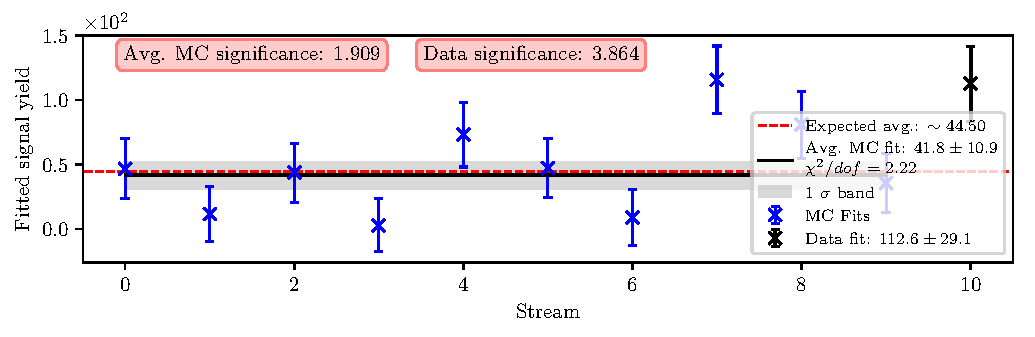
\includegraphics[width=\linewidth]{fig/sig_mKK_1}
	\caption{Signal fit result for the $1^{\mathrm{st}}$ $m_{KK}$ window for MC and data in the range $0.980  < m_{KK} < 1.011$.}
\end{figure} 

\begin{figure}[H]
	\centering
	\captionsetup{width=0.8\linewidth}
	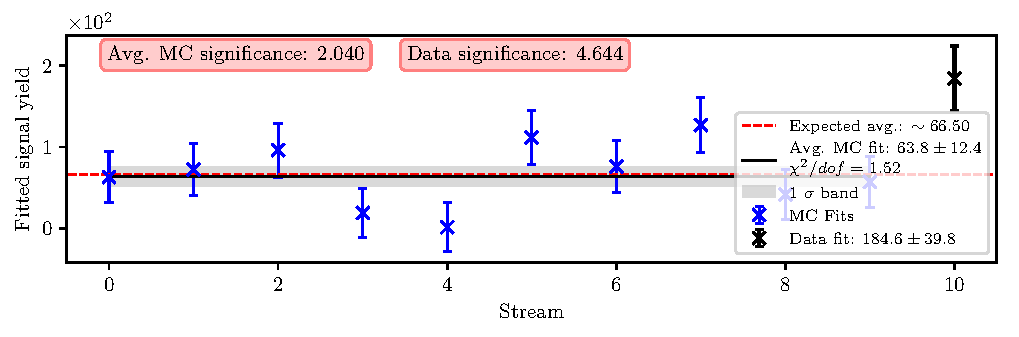
\includegraphics[width=\linewidth]{fig/sig_mKK_2}
	\caption{Signal fit result for the $2^{\mathrm{nd}}$ $m_{KK}$ window for MC and data in the range $1.011  < m_{KK} < 1.027$.}
\end{figure}

\begin{figure}[H]
	\centering
	\captionsetup{width=0.8\linewidth}
	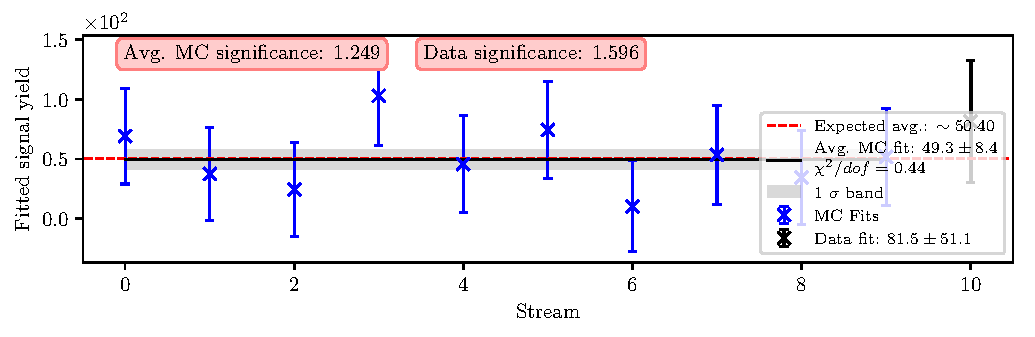
\includegraphics[width=\linewidth]{fig/sig_mKK_3}
	\caption{Signal fit result for the $3^{\mathrm{rd}}$ $m_{KK}$ window for MC and data in the range $1.027  < m_{KK} < 1.187$.}
\end{figure}

\begin{figure}[H]
	\centering
	\captionsetup{width=0.8\linewidth}
	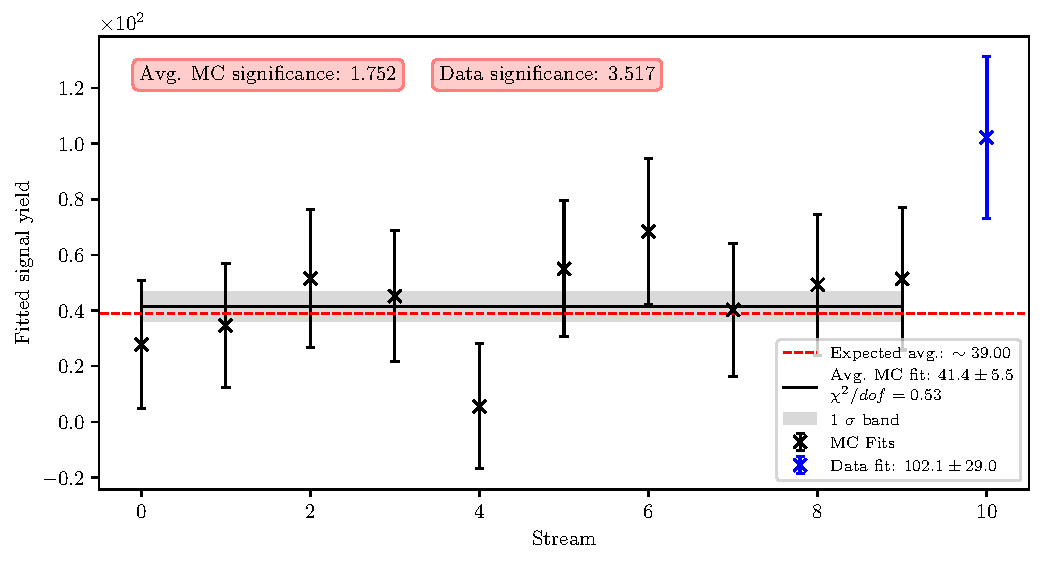
\includegraphics[width=\linewidth]{fig/sig_mKK_4}
	\caption{Signal fit result for the $4^{\mathrm{th}}$ $m_{KK}$ window for MC and data in the range $1.187  < m_{KK} < 1.342$.}
\end{figure}

\begin{figure}[H]
	\centering
	\captionsetup{width=0.8\linewidth}
	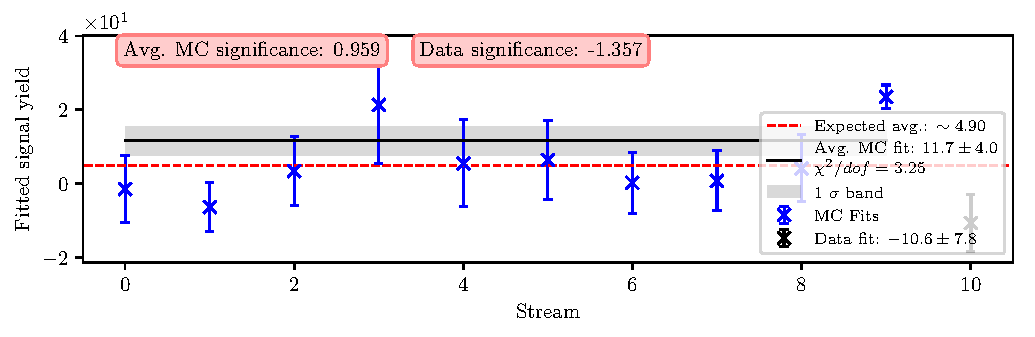
\includegraphics[width=\linewidth]{fig/sig_mKK_5}
	\caption{Signal fit result for the $5^{\mathrm{th}}$ $m_{KK}$ window for MC and data in the range $1.342  < m_{KK} < 1.497$.}
\end{figure}

\begin{figure}[H]
	\centering
	\captionsetup{width=0.8\linewidth}
	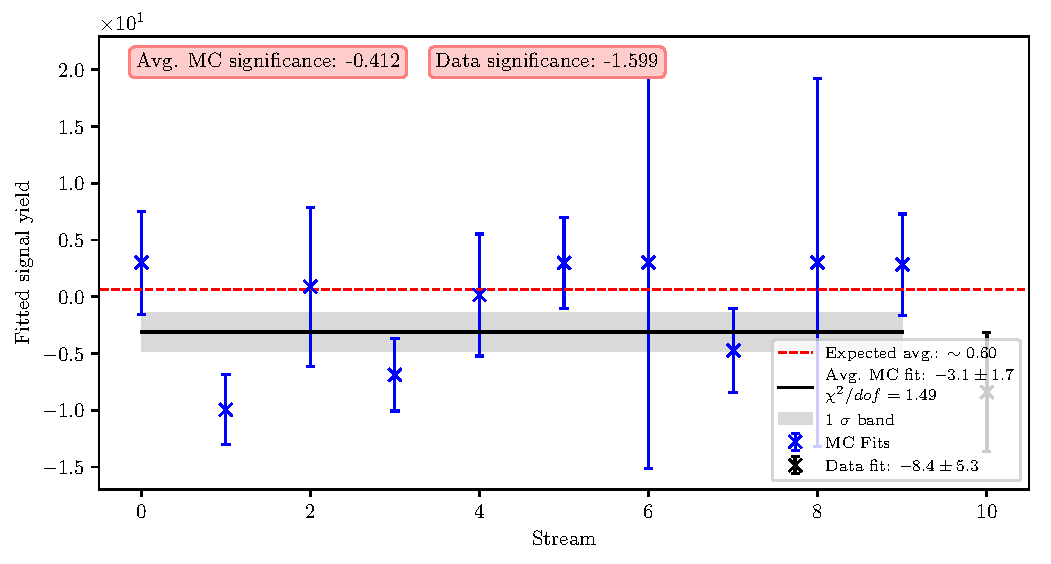
\includegraphics[width=\linewidth]{fig/sig_mKK_6}
	\caption{Signal fit result for the $6^{\mathrm{th}}$ $m_{KK}$ window for MC and data in the range $1.497  < m_{KK} < 1.647$.}
\end{figure}

\begin{figure}[H]
	\centering
	\captionsetup{width=0.8\linewidth}
	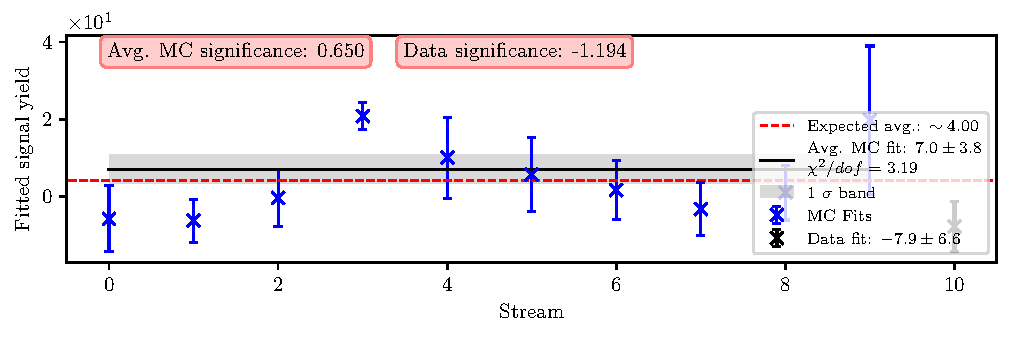
\includegraphics[width=\linewidth]{fig/sig_mKK_7}
	\caption{Signal fit result for the $7^{\mathrm{th}}$ $m_{KK}$ window for MC and data in the range $1.647  < m_{KK} < 1.850$.}
\end{figure}

\begin{figure}[H]
	\centering
	\captionsetup{width=0.8\linewidth}
	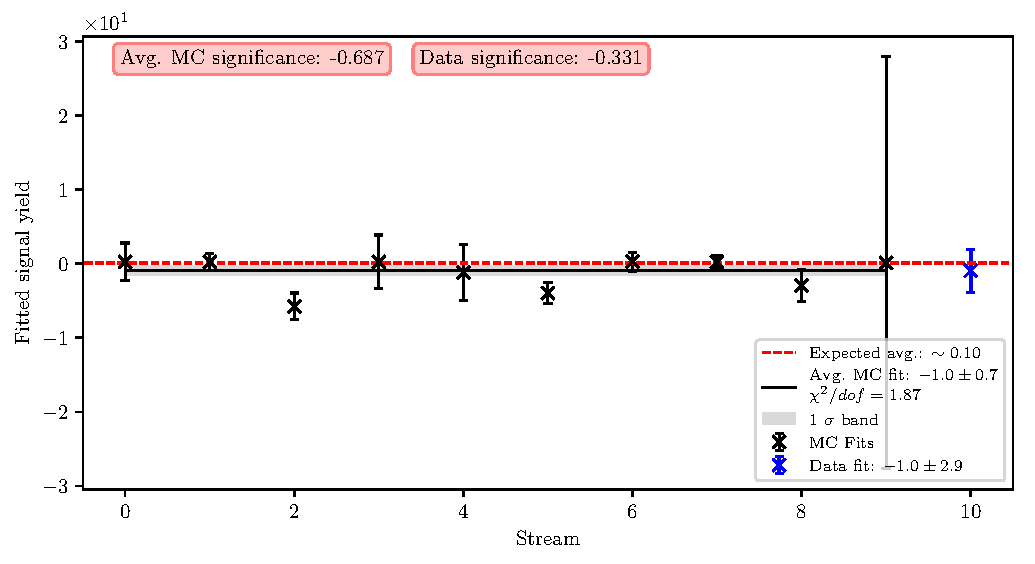
\includegraphics[width=\linewidth]{fig/sig_mKK_8}
	\caption{Signal fit result for the $8^{\mathrm{th}}$ $m_{KK}$ window for MC and data in the range $1.850  < m_{KK} < 1.880$.}
\end{figure}


\section{Signal Fits in \texorpdfstring{$q^2$}{q2}}
\label{sec:q2_plots}
\begin{figure}[H]
	\centering
	\captionsetup{width=0.8\linewidth}
	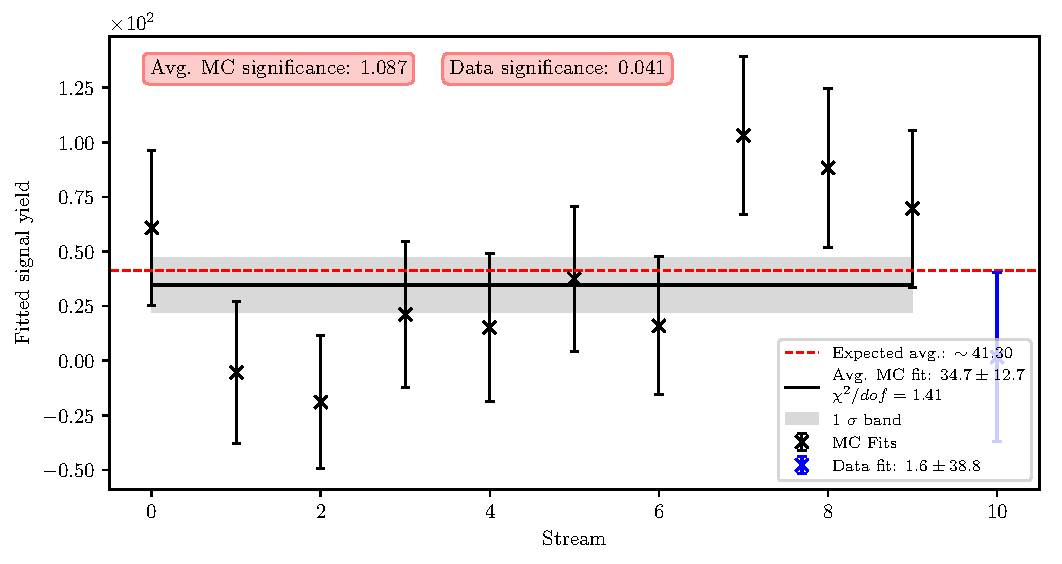
\includegraphics[width=\linewidth]{fig/sig_q2_1}
	\caption{Signal fit result for the $1^{\mathrm{st}}$ $q^2$ window for MC and data in the range $0.000  < q^2 < 2.250$.}
\end{figure} 

\begin{figure}[H]
	\centering
	\captionsetup{width=0.8\linewidth}
	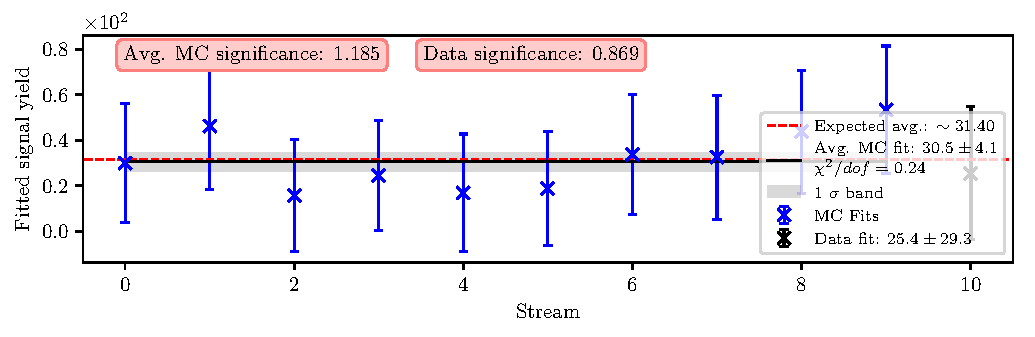
\includegraphics[width=\linewidth]{fig/sig_q2_2}
	\caption{Signal fit result for the $2^{\mathrm{nd}}$ $q^2$ window for MC and data in the range $2.250  < q^2 < 4.500$.}
\end{figure}

\begin{figure}[H]
	\centering
	\captionsetup{width=0.8\linewidth}
	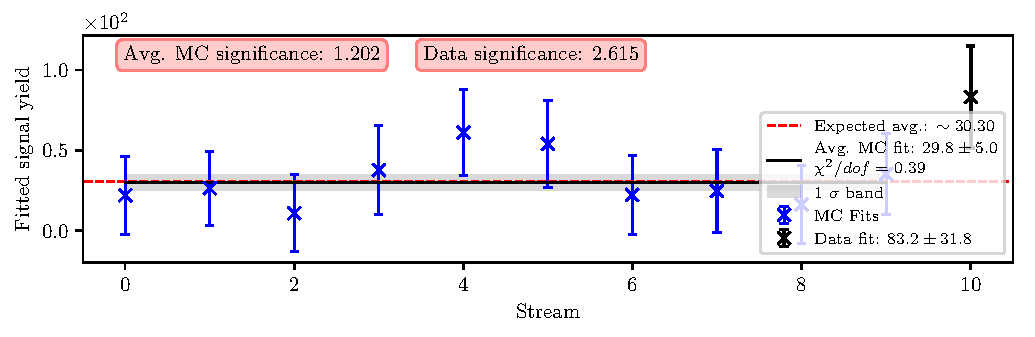
\includegraphics[width=\linewidth]{fig/sig_q2_3}
	\caption{Signal fit result for the $3^{\mathrm{rd}}$ $q^2$ window for MC and data in the range $4.500  < q^2 < 6.750$.}
\end{figure}

\begin{figure}[H]
	\centering
	\captionsetup{width=0.8\linewidth}
	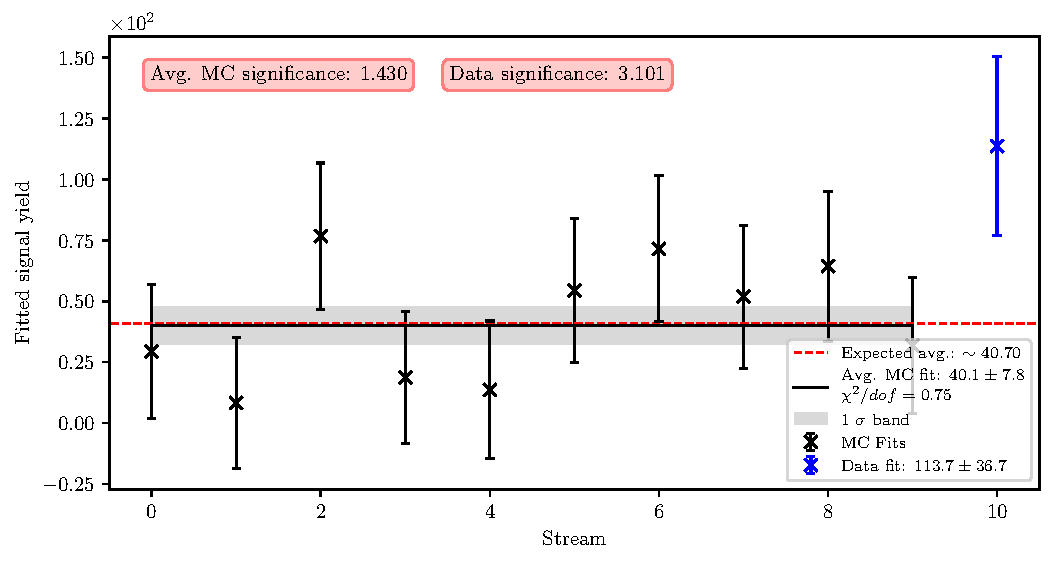
\includegraphics[width=\linewidth]{fig/sig_q2_4}
	\caption{Signal fit result for the $4^{\mathrm{th}}$ $q^2$ window for MC and data in the range $6.750  < q^2 < 9.000$.}
\end{figure}

\begin{figure}[H]
	\centering
	\captionsetup{width=0.8\linewidth}
	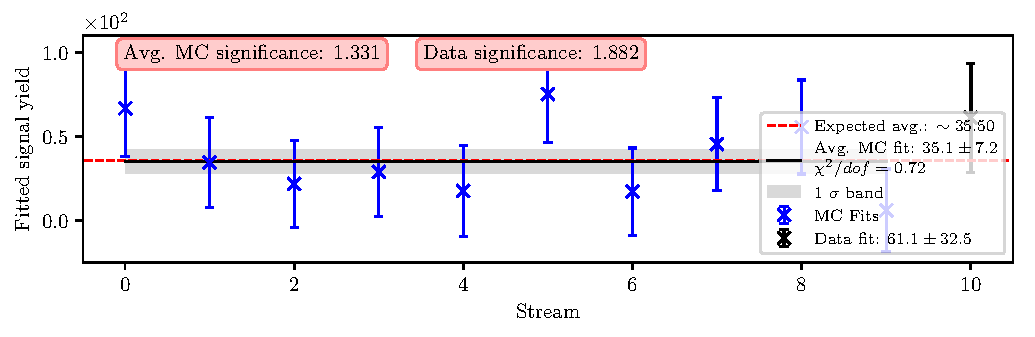
\includegraphics[width=\linewidth]{fig/sig_q2_5}
	\caption{Signal fit result for the $5^{\mathrm{th}}$ $q^2$ window for MC and data in the range $9.000  < q^2 < 11.250$.}
\end{figure}

\begin{figure}[H]
	\centering
	\captionsetup{width=0.8\linewidth}
	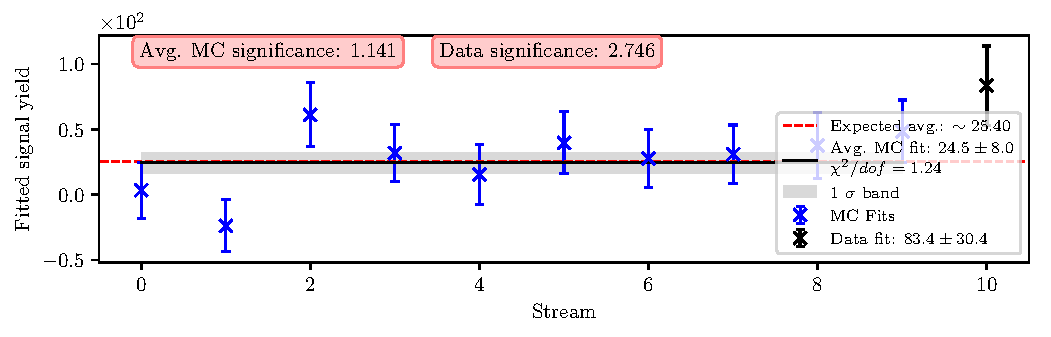
\includegraphics[width=\linewidth]{fig/sig_q2_6}
	\caption{Signal fit result for the $6^{\mathrm{th}}$ $q^2$ window for MC and data in the range $11.250  < q^2 < 13.500$.}
\end{figure}

\begin{figure}[H]
	\centering
	\captionsetup{width=0.8\linewidth}
	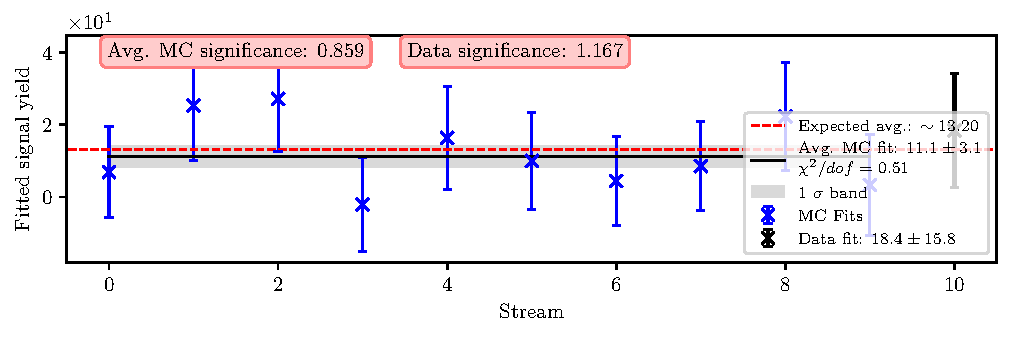
\includegraphics[width=\linewidth]{fig/sig_q2_7}
	\caption{Signal fit result for the $7^{\mathrm{th}}$ $q^2$ window for MC and data in the range $13.500  < q^2 < 15.750$.}
\end{figure}

\begin{figure}[H]
	\centering
	\captionsetup{width=0.8\linewidth}
	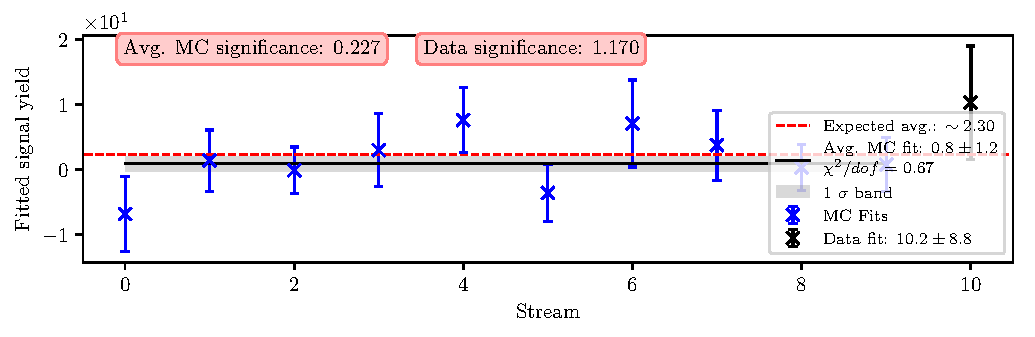
\includegraphics[width=\linewidth]{fig/sig_q2_8}
	\caption{Signal fit result for the $8^{\mathrm{th}}$ $q^2$ window for MC and data in the range $15.750  < q^2 < 18.000$.}
\end{figure}
